\section{Interaction classique champ-matière}

\subsection{Densité volumique de force électromagnétique}

Au niveau microscopique, on a la force de Lorentz $\vec{F}_{L}=q\left(\vec{E}+\vec{v}\wedge\vec{B}\right)$. Au niveau mésoscopique, la force moyenne $\vec{\d F}$ subie par les charges dans un élément de volume $\d\tau$ est alors
\begin{align}
    \vec{\d F}
    &=
    \sum_{\substack{\neq\text{ types}\\\text{de porteurs "k"}}}q_k\left(\vec{E}+\left\langle \vec{v}_k\right\rangle\wedge\vec{B}\right)n_k\d\tau\\
    &=
    \left(\left(\sum_{\text{"k"}}n_k q_k\right)\vec{E}+\left(\sum_{\text{"k"}}n_k q_k \left\langle\vec{v}_k\right\rangle\right)\wedge\vec{B}\right)\d\tau\\
    &=
    \left(\rho(\vec{r},t)\vec{E}+\vec{j}(\vec{r},t)\wedge\vec{B}\right)\d\tau\\
    &=
    \vec{f}_{\mathrm{vol}}\d\tau,
\end{align}
où
\begin{equation}
    \boxed{
        \vec{f}_{\mathrm{vol}}=\rho\vec{E}+\vec{j}\wedge\vec{B}.
    }
\end{equation}

\subsection{Puissance volumique fournie par le champ aux charges}

Au niveau microscopique, on a 
\begin{equation}
    P=\vec{F}_L\cdot\vec{v}=q\vec{E}\cdot\vec{v}.
\end{equation}
Au niveau microscopique, en notant $\d P_k$ la puissance reçue par les charges "k" dans $\d\tau$:
\begin{equation}
    \d P_k=
    q_k\vec{E}\cdot\left(n_k\d\tau\right)\left\langle \vec{v}_k\right\rangle.
\end{equation}
Ainsi, la puissance totale reçue par les charges dans $\d\tau$:
\begin{equation}
    \d P
    =
    \sum_{\neq \text{ "k"}}\d P_k
    =
    \left(\sum_{\neq \text{ "k"}}n_k q_k\left\langle v_k\right\rangle\right)\cdot\vec{E}\d\tau=\left(\vec{j}\cdot\vec{E}\right)\d\tau.
\end{equation}
La puissance volumique reçue par les charges de la part du champ électromagnétique est donc
\begin{equation}
    \boxed{
        P_{\mathrm{vol}}(\vec{r},t)=\vec{j}(\vec{r},t)\cdot\vec{E}(\vec{r},t).
    }
\end{equation}

\subsection{Cas des conducteurs ohmiques}
\subsubsection{Loi d'Ohm locale}

C'est une loi phénoménologique (pas comme les équations de Maxwell). L'idée est que si $\vec{E}=\vec{0}$, alors $\vec{j}=\vec{0}$ et si $\vec{E}\neq\vec{0}$ alors $\vec{j}\neq\vec{0}$. De plus, si $\left\lVert\vec{E}\right\rVert$ n'est \og pas trop grand\fg, et que $\left\lVert\vec{E}\right\rVert$ ne varie pas trop vite, alors $\vec{j}\propto\vec{E}$. On se donne alors la loi d'Ohm locale:
\begin{equation}
    \boxed{
        \vec{j}=\sigma\vec{E},
    }
\end{equation}
où $\sigma$ est la conductivité électrique, en $\si[]{\per\Omega\per\metre}$, ou bien
\begin{equation}
    \boxed{
        \vec{E}=\rho\vec{j},
    }
\end{equation}
avec $\rho=\sigma^{-1}$ est la résistivité électrique.

Ordre de grandeurs:
\begin{itemize}
    \item Cuivre: $\sigma\sim10^{7}\,\si{\per\ohm\per\metre}$;
    \item Silice (à 300$\si[]{\kelvin}$): $\sigma\sim10^{-4}\,\si{\per\ohm\per\metre}$;
    \item eau de mer: $\sigma\sim1\,\si{\per\ohm\per\metre}$.
\end{itemize}

\subsubsection{Loi de Joule locale}

La puissance volumique s'écrit
\begin{equation}
    \boxed{
        P_{\mathrm{vol}}=\vec{j}\cdot\vec{E}=\sigma E^{2}=\frac{j^{2}}{\sigma}.
    }
\end{equation}
On a $P_{\mathrm{vol}}>0$. Cette puissance est de nature mécanique (et non thermique), mais provoque un échauffement du réseau, par collisions des électrons de conduction sur les défauts du réseau cristallin. C'est l'effet Joule.

\subsubsection{Puissance disspée dans un conducteur ohmique cylindrique}

On de réfère à la Figure~\ref{fig:puissance_dissipee_conducteur_ohmique}. La puissance volumique s'écrit
\begin{equation}
    P_{\mathrm{vol}}=\vec{j}\cdot\vec{E}=\frac{j^{2}}{\sigma}=\frac{i^{2}}{\sigma(\pi a)^{2}}=\mathrm{constante}.
\end{equation}
La puissance par effet Joule est donc 
\begin{equation}
    P_{\mathrm{Joule}}=P_{\mathrm{vol}}\times \pi a^{2}l=\frac{i^{2}l}{\sigma(\pi a)^{2}}=R i^{2},
\end{equation}
avec 
\begin{equation}
    \boxed{
        R=\frac{l}{\sigma\pi a^{2}}=\frac{l}{\sigma S}.
    }
\end{equation}

\begin{figure}
    \centering
    \tikzsetnextfilename{puissance_dissipee_conducteur_ohmique}
    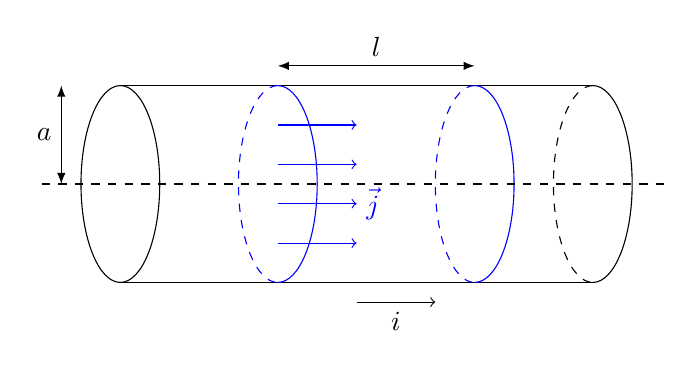
\begin{tikzpicture}[scale=1]  
        % \helpgrid{3}{3}
        \draw (0,0) ellipse (0.5 and 1.25);
        \draw (0,1.25) --++ (6,0);
        \draw (0,-1.25) --++ (6,0);
        \draw (6,1.25) arc (90:-90:0.5 and 1.25);
        \draw [dashed] (6,1.25) arc (90:-90:-0.5 and 1.25);
        \draw [blue, dashed] (4.5,1.25) arc (90:-90:-0.5 and 1.25);
        \draw [blue, dashed] (2,1.25) arc (90:-90:-0.5 and 1.25);
        \draw [blue] (2,1.25) arc (90:-90:0.5 and 1.25);
        \draw [blue] (4.5,1.25) arc (90:-90:0.5 and 1.25);
        \draw [latex-latex] (2,1.5)--(4.5,1.5) node [above, midway] {$l$};
        \draw [latex-latex] (-0.75,0)--(-0.75,1.25) node [left, midway] {$a$};        
        \draw[dashed] (-1,0) -- (7,0);
        \draw[->] (3,-1.5) --++ (1,0) node [midway, below] {$i$};
        \draw[draw=blue,->] (2,0.25) --++ (1,0);
        \draw[draw=blue,->] (2,0.75) --++ (1,0);
        \draw[text=blue,draw=blue,->] (2,-0.25) --++ (1,0) node [pos=1, right] {$\vec{j}$};
        \draw[draw=blue,->] (2,-0.75) --++ (1,0);
    \end{tikzpicture}
    \caption{Puissance dissipée dans un conducteur cylindrique.}    
    \label{fig:puissance_dissipee_conducteur_ohmique}
\end{figure}